
\section{Užívateľská príručka}
Program sa spúšťa prostredníctvom vývojového prostredia Qt a beží ako natívna aplikácia. K svojmu plnohodnotnému fungovaniu vyžaduje nadviazanie spojenia so simulátorom Kobuki (alebo s reálnym robotom), ktorý mu poskytuje potrebné dáta senzoriky a prijíma príkazy pre motory. Všetky detaily týkajúce sa prerekvizít, prvotného nastavenia projektových súborov a samotnej inštalácie sú podrobne popísané v samostatnom inštalačnom manuáli k projektu.

Softvér disponuje grafickým užívateľským rozhraním určeným na zadávanie cieľov a spúšťanie vnútorných procesov robota.

\begin{figure}[h]
    \centering
    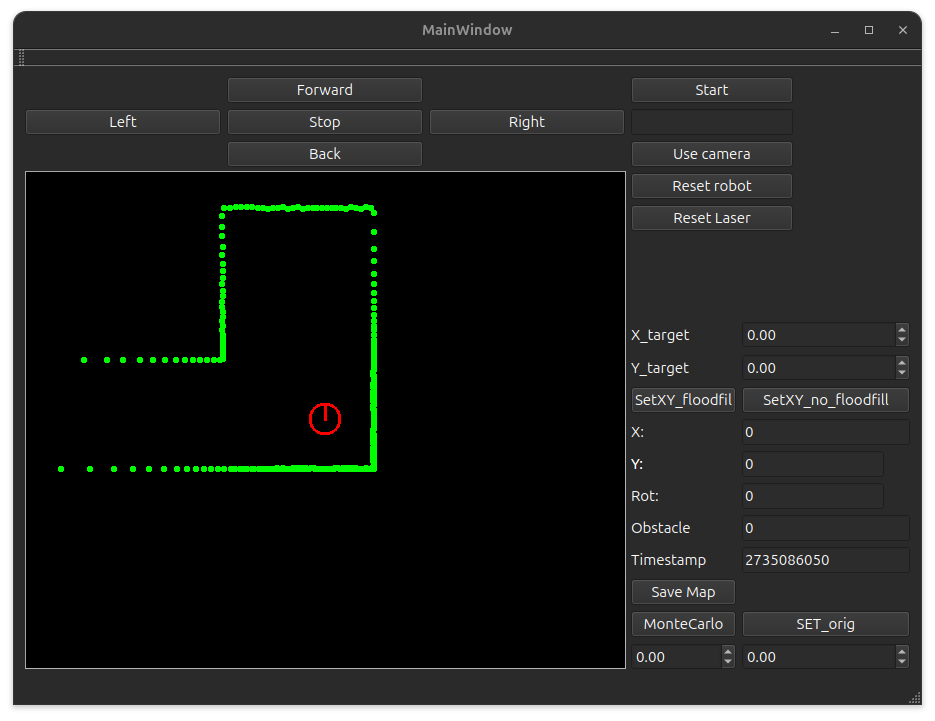
\includegraphics[width=1\textwidth]{img/MainWindow.png}
    \caption{Ukážka užívateľského rozhrania}
    \label{fig:gui}
\end{figure}

Na obrázku \ref{fig:gui} je znázornené užívateľské rozhranie programu. V strednej časti je zobrazený robot a body, ktoré sú detekované pomocou lidaru. V hornej časti sa nachádzajú pôvodné tlačidlá pre ovládanie robota (\texttt{Forward, Backward, Left, Right, Stop}) a v pravom hornom rohu sú tlačidlá Start, Use camera, Reset robot, Reset Laser. Tlačidlom Start sa spúšťa hlavný cyklus programu a pripojenie sa k IP adrese robota. Textové polia \texttt{X\_target} a \texttt{Y\_target} slúžia na zadávanie súradníc cieľa, ktorý sa načíta do poľa súradníc po stlačení tlačidla \texttt{SetXY\_no\_floodfill}, ktoré zapíše body priamo do poľa, alebo \texttt{SetXY\_floodfill}, ktoré zavolá floodfill algoritmus. Textové polia X, Y a Rot zobrazujú aktuálnu pozíciu a orientáciu robota. Obstacle signalizuje, či sa robot nachádza v móde vyhýbania sa prekážkám. Timestamp zobrazuje aktuálnu časovú vzorku. Tlačidlo \texttt{Save Map} umožňuje uložiť aktuálne zmapovaný priestor do súboru. Tlačidlo \texttt{Monte Carlo} spustí lokalizačný algoritmus Monte Carlo, ktorého výstup sa zobrazuje v konzole. Tlačidlo \texttt{SET\_orig} nastavuje robotu jeho aktuálnu pozíciu na súradnice X a Y z textových polí pod ním.

\begin{figure}[h]
    \centering
    \includegraphics[width=0.7\textwidth]{img/MapVis.png}
    \caption{Ukážka vizualizácie mapy}
    \label{fig:mapvisualizer}    
\end{figure}

Na obrázku \ref{fig:mapvisualizer} je zobrazené okno vizualizácie mapy, ktoré sa zobrazí po stlačení tlačidla \texttt{Start}. V tomto okne je zobrazená mapa, ktorú robot vytvára počas pohybu v priestore. Biele body reprezentujú body detekované lidarom, čierny podklad reprezentuje voľný priestor.




\newpage
\section{Úloha 1: Lokalizácia a polohovanie robota v prostredí}
Táto kapitola popisuje funkcie pre bezkolízny priamočiary pohyb a sledovanie vlastnej polohy na základe odometrie.

\subsection{Lokalizácia (updateOdometry)}
Ide o základný stavebný kameň lokalizácie, ktorý sa stará o presné počítanie polohy $x$, $y$ a natočenia z enkodérov a gyroskopu robota. Výpočet využíva diferencie hodnôt medzi jednotlivými volaniami. 
Enkodéry vrátia delta polohy na ľavom a pravom kolese, z ktorých je vypočítaná priemerná prejdená vzdialenosť (translácia).

\subsection{Pohyb smerom na cieľ}
Bezpečný pohyb po priestore zaručuje trajektória riadená pomocou metódy \newline \noindent\texttt{updateArcTrajectory}, pokiaľ lidar nezaregistroval prekážku a teda flag detekcie prekážky \texttt{obstacle\_detected = false}.
Algoritmus skontroluje vzdialenosť do cieľa prostredníctvom pomocných matematických funkcií \texttt{calculateAngleToTarget}, ktorá Nájde najkratší uhol medzi aktuálnou rovinou ($x\_curr, y\_curr$) a koncovým cieľom použitím arkustangens (\texttt{atan2}) a \texttt{normalizeAngle}, ktorá pripočítava alebo odpočítava konštantu $2\pi$, aby uhol zotrval vo formáte $(-\pi, \pi \rangle$.


O pootočenie okolo osi Z za behu do daného smeru sa stará funkcia \texttt{piRegulator}. Do regulátora vstupuje uhlová odchýlka (\texttt{heading\_error}) a na základe $K_p$ (Zosilnenie proporcionálnej zložky) a $K_i$ (Zosilnenie integračnej zložky) konštánt sa vracia rýchlosť natáčania s anti-windup podmienkou (ohraničenie akumulovanej chyby v integrátore). 
Zároveň kvôli stabilite je volaná funkcia \texttt{applySpeedRamp}, ktorá implementuje S-krivku (zrýchľovací/spomaľovací profil polynomiálneho radu) pre elimináciu trhania robota, stabilný a plynulý priebeh zmeny rýchlosti pohybu.



\newpage
\section{Úloha 2: Navigácia a vyhýbanie sa prekážkam}
Ak sa robot po ceste k cieľu stretne s objektom, prechádza plynulo do módu vyhýbania a obchádzania stien. 

\subsection{Lidar a prekážky}
Lidar vracia veľké množstvo bodových meraní v rôznych uhloch. Vzorka merania pokrýva plné okolie robota. Úlohou funkcie \texttt{obstacleDetector} je tieto body normalizovať a vyhodnotiť ich na základe hraničných hodnôt vzdialeností (tzv. \textit{threshold\_mm} a \textit{hysteresis\_mm}). Setuje bool hodnotu \texttt{obstacle\_detected = true}, čím signalizuje systému že nemôže pokračovať v pôvodne naplánovanej trajektórii k cielu bez kolízie a mení interný stav pre výber trasy.

Na optimalizáciu je priestor okolo robota (360 stupňov) rozdelených na 80 sektorov, z ktorých každý predstavuje uhol $4,5^\circ$. Metóda \texttt{updateLidarSegments} v spolupráci s \texttt{rotateLidarSegmentsBySteps} v \texttt{updateOdometry} vykonáva stabilizáciu tohto mapovaného okolia - tzn. fixujú dáta napriek uhlu natočenia robota použitím hodnôt iterácií delty z gyroskopu a rotujú kandidátske pole, takže index poľa prislúcha v určitom okamihu absolútnemu uhlu voči globálnej rovine, a nie k osi robota.

\subsection{Hľadanie cesty na obchádzanie prekážky}
Vo chvíli detekovania prekážky musí robot zmeniť svoj cieľový smer. Metóda \texttt{candidateDirection} prehľadáva prekážkové segmenty. Identifikuje priechodznosti kandidátskych smerov, na ktoré nasadzuje prispôsobený algoritmus ohodnotenia (Fitness).

Konkrétna implementácia fitness hodnotí vhodnosť daného voľného smeru:
\begin{equation}
    \text{Fitness} = \mu_1 \cdot \text{finish\_distance} + \mu_2 \cdot \text{rotate\_distance} + \mu_3 \cdot \text{change\_distance}
\end{equation}
kde \texttt{finish\_distance} je veľkosť uhla medzi kandidátskym bodom a cieľovým bodom, \texttt{rotate\_distance} je potrebná výchylka robota, \texttt{change\_distance} je vzdialenosť pri zmene ohodnoteného bodu z predošlého výpočtu. Slúži ako histeréza, aby robot stabilne držal aktuálne zvolený smer vyhýbania sa a nemenil smery pri identickom fitness ohodnotení pravého či ľavého smeru obchádzania, $\mu_1$, $\mu_2$ a $\mu_3$ sú váhy, ktoré určujú dôležitosť jednotlivých faktorov v celkovej fitness funkcii. Kandidát s najnižšou hodnotou fitness sa ukladá ako najlepší kandidát. 


\subsection{Vyhýbacie manévre}
V stave vyhýbania sa prekážke robot riadi \texttt{rotationspeed} opätovným využitím funkcie PI regulácie \texttt{piRegulator}, avšak tento raz chybu vyčísluje na základe uhlovej odchýlky vypočítanej pre zvolený kandidátsky smer z funkcie \texttt{candidateDirection()}.




\section{Úloha 3: Mapovanie}
Mapovanie prebieha od spustenia programu a počas celého behu. Lidarové dáta sa na základe aktuálnej polohy robota a jeho orientácie transformujú do dvojrozmernej mapy. Mapa je zobrazená na obrázku \ref{fig:mapvisualizer} a je aktualizovaná v reálnom čase.

\subsection{Vytváranie mapy - mapping.cpp}
Mapa sa inicializuje ako pole s rozmermi 1362 x 1204, čo je dvojnásobok rozmerov mapy v pixeloch (681 x 602) pre zabezpečenie dostatočného priestoru, v prípade, že robot nebude začínať v bode (0, 0). Každý pixel mapy zodpovedá 1 centimetru v reálnom svete. Mapa je reprezentovaná ako pole, kde 0 značí voľný priestor a 255 značí detekovaný objekt alebo stenu. Tieto hodnoty boli zvolené kvôli jednoduchosti vizualizácie, ktorá je popísaná v ďalšej podkapitole.

Metóda \texttt{onLidarData} pre každú vzorku lidarových dát rozhoduje o platnosti merania a následne volá metódu \texttt{updateMapFromLidar}, ktorá aktualizuje mapu. Na základe aktuálnej pozície robota a jeho orientácie sa body z lidaru transformujú do globálnych súradníc a aktualizujú sa hodnoty v mape. 

Na kompenzáciu nepresností v meraní počas pohybu robota sa využíva funkcia lineárna interpolácia bodov, ktorá sa vykonáva v metóde \texttt{interpolatePose}. Táto metóda interpoluje pozíciu meraných bodov v čase, aby sa zohľadnili zmeny v polohe robota medzi jednotlivými meraniami lidaru. \texttt{interpolatePose} využíva časové vzorky z odometrie a lidaru, ktorých synchronizácia prebieha v metóde \texttt{liftLidarTimestamp}. Táto metóda ošetruje pretečenie hodnoty časovej vzorky lidaru a vyberá najlepšie zodpovedajúci časový interval. Metóda \texttt{unwrapRobotTimestamp} zabezpečuje, že po sebe nasledujúce časové vzorky ošetrené proti pretečeniu majú narastajúce hodnoty času, aby bolo možné správne interpolovať. Pre zaznamenávanie histórie pozícií pre interpoláciu sa využíva štruktúra \texttt{pose\_history}, ktorá je vytváraná volaním metódy \texttt{recordPose}. 

Metóda \texttt{saveMapToFile} umožňuje uložiť aktuálnu mapu do textového súboru. Táto metóda je volaná po stlačení tlačidla \texttt{Save Map} v užívateľskom rozhraní. 


\subsection{Vizualizácia mapy - mapvisualizer.cpp}

Trieda \texttt{MapVisualizer} sa stará o vizualizáciu mapy v reálnom čase. Mapa je zobrazovaná ako v okne užívateľského rozhrania, ako je zobrazené na obrázku \ref{fig:mapvisualizer}. Volanie metódy \texttt{onMapUpdated} zabezpečuje aktualizáciu zobrazenia mapy vždy, keď sa mapa aktualizuje. Dáta na vykreslenie mapy sú získané z triedy \texttt{Mapping} pomocou metódy \texttt{getGridImage}, ktorá vracia maticu z knižnice OpenCV.



\newpage
\section{Úloha 4: Globálna navigácia po známej mape (Floodfill)}
Táto časť popisuje spôsob implementácie globálnej navigácie, ktorá využíva mapu prekážok a na ktorej sa robot dokáže lokalizovať. Algoritmus floodfill poskytuje robustnejší postup na vyhýbanie sa prekážkam na mape, čím priamo nahrádza lokálnu navigáciu a algoritmus obchádzania prekážok z úlohy 2 pre známe prekážky.

\subsection{Transformácie mapy a robota}
Základným predpokladom úspešnej dráhy je znalosť vlastnej polohy a pozície na mape. V tejto chvíli je manuálne vložená hodnota z lokálneho súradnicového systému robota (0, 0). Do softvéru vstupujú transformácie, ktoré umožňujú interpolovať a prepisovať reálne pozície robota a polohy jednotlivých pixelov (hodnôt v mape charakterov) mapy zobrazených cez mriežku (grid). Týmito transformáciami vieme určiť jednoznačnú pozíciu poľa a vzdialenosti prvkov.

\subsection{Vytvorenie Waypointov pomocou Breadth-First Search (BFS)}

Celá voľná zóna je reprezentovaná pre algoritmus ako sieť prepojených bodov v gride (t.j. hrany medzi poliami mapy nemajú rôznu dĺžku). Graf hľadá cestu naprieč mapou tak, že sa v iteratívnych prechodoch značí susedné bunky (či už steny alebo voľný priestor, aby viackát neprehľadal ten istý pixel) na okolité susedné vrcholy, až kým nenatrafí na character F (finish). 

Výstupom tohto algoritmu sú \textit{waypointy} (určené lámaním trajektórie), inak zlomové body na mape. Tie sú generované ako trasa k samotnému koncu a sú zasielané ako sústava postupných cieľov \texttt{x\_target} a \texttt{y\_target}. 

\subsection{Sledovanie Waypointov s reflexiou neočakávaných prekážok}
Akonáhle dostane štruktúra \texttt{robot} a jeho metódy na starosť tieto waypointy, začne ich sledovať použitím lokálneho kontroléru popísaného v Úlohe 1 (presun v móde \texttt{obstacle\_detected = false}). Robot nasleduje zadané úseky, no zároveň aktívne stráži okolie cez lidar pre prípad nečakaných prekážok. Ak sa táto prekážka obajaví, robot nastaví flag \texttt{obstacle\_detected = true} a prejde do módu vyhýbania sa prekážkam, pričom bude pokračovať v sledovaní aktuálneho waypointu. Po úspešnom obídení prekážky sa vráti do módu štandardného pohybu a bude pokračovať v ceste k waypointu, až kým nedosiahne cieľ.



\section{Úloha 5: Monte Carlo lokalizácia (MCL)}
V prípadoch, keď poloha robota na mape nie je jednoznačne určená alebo po strate presnosti odometrie, kvôli driftu gyroskopu alebo prešmykovaniu kolies systém pristupuje k proaktívnemu hľadaniu vlastnej globálnej polohy za pomoci Monte Carlo lokalizácie (často označovanej aj ako Particle Filter).

Mechanizmus využíva samostatné asynchrónne vlákno (trieda \texttt{MonteCarlo}), ktoré simuluje možné hypotézy o polohe robota v podobe mračna častíc (particles). Algoritmus zbieha slučku viacerých výpočtových subrutín, až kým nepotvrdí zistenie svojej vlastnej polohy (\texttt{foundMyself = true}).

\subsection{Inicializácia hypotéz}
Na začiatku sa pomocou funkcie \texttt{initParticlesGlobal} vo voľnom priestore, ktoré robot extrahuje z mapy znakov \texttt{finalMap.txt}, rozmiestni špecifikovaný počet častíc (štandardne v zadaní 100). Voľnosť náhodne vybranej bunky, do ktorej sa vygeneruje častica sa overí pomocou funkcie \texttt{isFreeSpace()}). V každej iterácii sa vygeneruje náhodná počiatočná pozícia častice $x$, $y$ a náhodná rotácia $\theta$ s počiatočnou váhou a chybou $error = 0$.

\subsection{Ohodnocovanie častíc}
V hlavnej slučke MCL systému sa pre každú hypotetickú časticu porovnávajú dáta namerané reálnym Lidarom na robote s teoretickým modelom vzdialeností načítaným z textového súboru \texttt{distanceMap.txt}. Častice vrhajú virtuálne lúče od seba von a prepočítavajú sa na mriežku senzorických polí prostredníctvom pomocnej metódy \texttt{transform()}. Súčty vzdialeností od steny penalizujú celkovú presnosť (\texttt{p.error}) danej častice. Ak častica vygeneruje lúč smerujúci von z mapy, obdrží penalizáciu ($+200$). Celková metrika vzdialeností je zároveň uložená v častici do hodnôt \texttt{weight}.

\subsection{Ruletový výber}
Filtrovací systém ďalej realokuje nové generácie častíc cez metódu opakovaného prevzorkovania. Častica, ktorá mala veľkú chybu (a bola označená ako veľmi nepravdepodobná varianta polohy) má malú šancu na výber do ďalšej generácie. Častica z menšou chybou má pri ruletovom výbere vyššiu váhu, a teda vyššiu pravdepodobnosť výberu.

Nasleduje filter \texttt{cutoff()}, ktorý orezáva častice nachádzajúce sa v stenách, a častice errorom nad hranicu $10000.0$. Tie sú automaticky zahodené a nanovo inicializované rovnako ako v inicializačnej metóde \texttt{initParticlesGlobal()}.

\subsection{Pohyb a pridávanie šumu}
Pre zlepšenie presnosti lokalizácie sa pred ďalšou iteráciou volá metóda \texttt{noise()}. Pridáva každej častici náhodnú hodnotu z Gaussovho pravdepodobnostného rozdelenia k súradniciam a uhlu. To zabraňuje tomu, aby sa všetky dobré častice ustálili v identickom bode. V poslednom kroku metóda \texttt{move()} upravuje polohu častice o rotáciu a transláciu prekopírovaným predchádzujúcim pohybom robota. 
